
%%%%%%%%%%%%%%%%%%%%%%% file typeinst.tex %%%%%%%%%%%%%%%%%%%%%%%%%
%
% This is the LaTeX source for the instructions to authors using
% the LaTeX document class 'llncs.cls' for contributions to
% the Lecture Notes in Computer Sciences series.
% http://www.springer.com/lncs       Springer Heidelberg 2006/05/04
%
% It may be used as a template for your own input - copy it
% to a new file with a new name and use it as the basis
% for your article.
%
% NB: the document class 'llncs' has its own and detailed documentation, see
% ftp://ftp.springer.de/data/pubftp/pub/tex/latex/llncs/latex2e/llncsdoc.pdf
%
%%%%%%%%%%%%%%%%%%%%%%%%%%%%%%%%%%%%%%%%%%%%%%%%%%%%%%%%%%%%%%%%%%%


\documentclass[runningheads,a4paper]{llncs}

\usepackage{amssymb}
\setcounter{tocdepth}{3}
\usepackage{graphicx}
\usepackage{booktabs}
\usepackage{times}
\usepackage{epsfig}
\usepackage{amsmath}
\usepackage{amssymb}
\usepackage{multirow}

\usepackage{url}
\urldef{\mailsa}\path|{alfred.hofmann, ursula.barth, ingrid.haas, frank.holzwarth,|
\urldef{\mailsb}\path|anna.kramer, leonie.kunz, christine.reiss, nicole.sator,|
\urldef{\mailsc}\path|erika.siebert-cole, peter.strasser, lncs}@springer.com|
\newcommand{\keywords}[1]{\par\addvspace\baselineskip
\noindent\keywordname\enspace\ignorespaces#1}

% macros for referencing figures, tables, equations and sections
\newcommand{\fref}[1]{Figure~\ref{#1}}
\newcommand{\eref}[1]{(\ref{#1})}
\newcommand{\tref}[1]{Table~\ref{#1}}
\newcommand{\sref}[1]{Section~\ref{#1}}
\newcommand{\aref}[1]{Algorithm~\ref{#1}}

%\newcommand{\toprule}{\hline\noalign{\smallskip}}
%\newcommand{\midrule}[1]{\cline{#1}\noalign{\smallskip}}
%\newcommand{\bottomrule}{\hline\noalign{\smallskip}}

% maths macros
\def\G{G}
\def\Gx{G_x}
\def\Gy{G_y}
\def\Gxx{G_{xx}}
\def\Gxy{G_{xy}} \def\Gyx{G_{yx}}
\def\Gyy{G_{yy}}
\def\Ix{I_x}
\def\Iy{I_y}
\def\Ixsqr{I_{x^2}}
\def\Iysqr{I_{y^2}}
\def\Ixx{I_{xx}}
\def\Ixy{I_{xy}}
\def\Iyy{I_{yy}}
\def\dtcwt{DT-$\mathbb{C}$WT}
\def\figpath{./figs}
\def\ie{i.e.}
\def\eg{e.g.}

% command for adding inline comment to text
\newcommand{\comment}[1]{}

\begin{document}

\mainmatter  % start of an individual contribution

% first the title is needed
\title{Estimating Orientation of Curvilinear Structure in Medical Images}

% a short form should be given in case it is too long for the running head
\titlerunning{Estimating Orientation in Medical Images}

% the name(s) of the author(s) follow(s) next
%
% NB: Chinese authors should write their first names(s) in front of
% their surnames. This ensures that the names appear correctly in
% the running heads and the author index.
%
\author{*}%
%\thanks{Please note that the LNCS Editorial assumes that all authors have used
%the western naming convention, with given names preceding surnames. This determines
%the structure of the names in the running heads and the author index.}%
%\and Ursula Barth\and Ingrid Haas\and Frank Holzwarth\and\\
%Anna Kramer\and Leonie Kunz\and Christine Rei\ss\and\\
%Nicole Sator\and Erika Siebert-Cole\and Peter Stra\ss er}
%
%\authorrunning{Lecture Notes in Computer Science: Authors' Instructions}
% (feature abused for this document to repeat the title also on left hand pages)

% the affiliations are given next; don't give your e-mail address
% unless you accept that it will be published
\institute{*}
%Tiergartenstr. 17, 69121 Heidelberg, Germany\\
%\mailsa\\
%\mailsb\\
%\mailsc\\
%\url{http://www.springer.com/lncs}}

%
% NB: a more complex sample for affiliations and the mapping to the
% corresponding authors can be found in the file "llncs.dem"
% (search for the string "\mainmatter" where a contribution starts).
% "llncs.dem" accompanies the document class "llncs.cls".
%

\toctitle{Lecture Notes in Computer Science}
\tocauthor{ }
\maketitle


\begin{abstract}
Estimating orientation of image structure underpins applications including digital mammography, retinography, fingerprint analysis and many more. We consider different choices of filter bank including those based on first and second derivatives, the Monogenic Signal and the Dual Tree Complex Wavelet Transform (\dtcwt). We then investigate how standard regressors (linear regression, Boosting and Random Forests) may be adapted to use the responses to these filter banks in order to predict orientation of image structure. For a quantitative evaluation, we use synthetic images based on mammograms and the publicly available DRIVE database of retinal images, and show that the combination of Random Forest regression with \dtcwt~features offers superior accuracy though at a cost in efficiency.
\keywords{We would like to encourage you to list your keywords within
the abstract section}
\end{abstract}

\section{Introduction}
\label{s:introduction}
Curvilinear structures are important in many applications of computer vision, including aerial image analysis (roads, rivers, railways), fingerprint analysis (ridges) and medical image analysis (blood vessels, ducts). As a result, there is an extensive literature on detecting such structure~\cite{Papari_Petkov_IVC11,Staal_etal_TMI04,Ricci_Perfetti_TMI07}. The literature on estimating the local orientation of curvilinear structure is more limited though the problem is equally important, with applications in low-level and intermediate-level processing and high-level image interpretation.

In low-level processing, local orientation is used to steer computation, for example in non-maximal suppression for centre-line detection~\cite{Sonka_99}, profile extraction for structure classification~\cite{Zwiggelaar_etal_TMI04} and anisotropic diffusion~\cite{Perona_PAMI90}.  In intermediate-level processing, local orientation is used in grouping and tracking for extracting curvilinear features~\cite{Aylward_Bullitt_TMI02,Staal_etal_TMI04}.

Applications of local orientation in high-level interpretation are more diverse. For example, in retinography (\fref{f:retinography}), the rate of change of orientation (\ie~tortuosity) of blood vessels can serve as a diagnostic indicator of vascular disease~\cite{Hart_etal_IJMI99}. Similarly, in x-ray mammography, local orientation can be used to detect the patterns of radiating curvilinear structures (known as spicules) that are often associated with malignant lesions~\cite{Zwiggelaar_etal_MIA99,Karssemeijer_teBrake_TMI96,Rangayyan_Ayres_MBEC06}. In automatic fingerprint analysis, typically the local orientations of ridges are used, to create an orientation field~\cite{Bazen_Gerez_TPAMI02,Mei_etal_IVC09} which is parameterised (\eg~via `phase portraits'~\cite{Li_etal_PR06} or polynomial approximation~\cite{Gu_etal_PR04}) as a basis for recognition.


\begin{figure}[t]
\centering
\begin{tabular}{@{}c c c@{}}
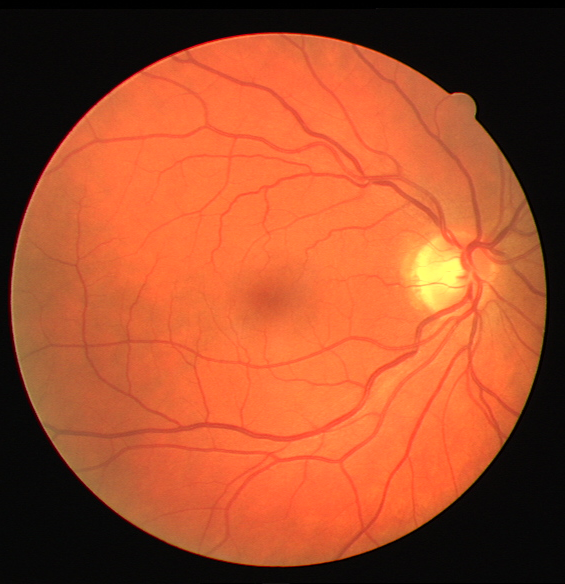
\includegraphics[width=0.3\columnwidth]{\figpath/retina/02_test} &
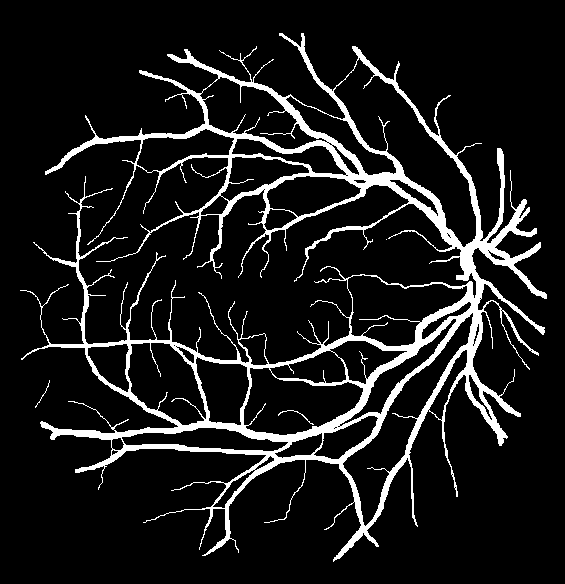
\includegraphics[width=0.3\columnwidth]{\figpath/retina/02_manual1_pos} &
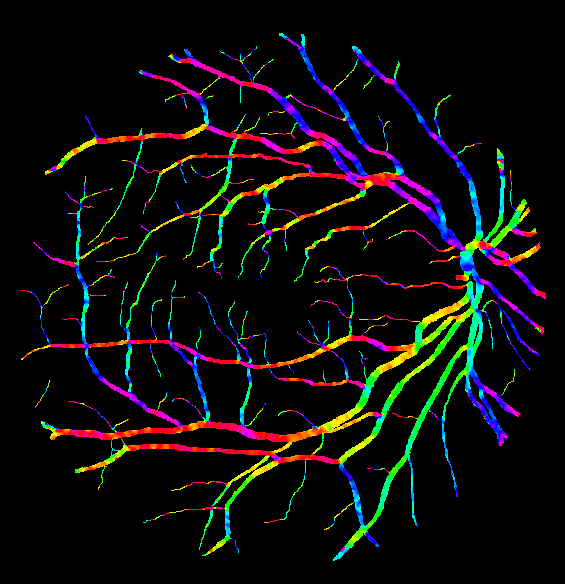
\includegraphics[width=0.3\columnwidth]{\figpath/retina/002_orientation_masked} \\
%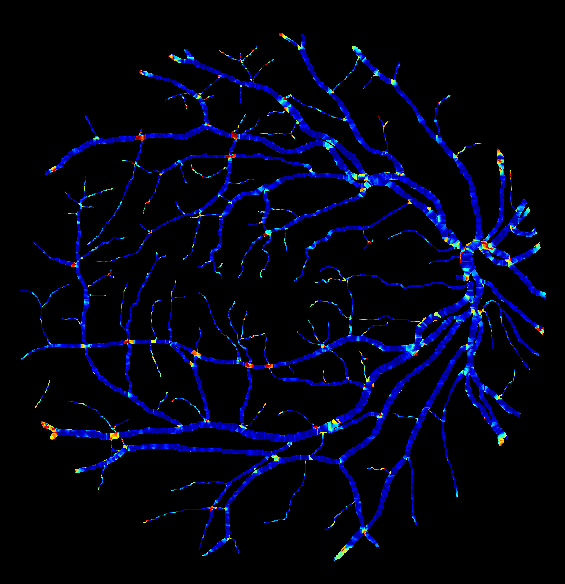
\includegraphics[height=0.15\textheight]{\figpath/retina/002_abs_error} \\
(a) & (b) & (c) \\
\noalign{\smallskip}
\end{tabular}
%
\caption{Estimating orientation in retinography: %
(a) input image; %
(b) ground truth mask indicating pixels belonging to a vessel; %
(c) orientation (indicated by colour) estimated using linear regression over \dtcwt~features. The mask was not used to estimate orientation. %
%(c) magnitude of error (note the regions of high error at points of bifurcation.)
}
\label{f:retinography}
\end{figure}


In this paper we revisit the problem of orientation estimation, reviewing the basic theory, extending the state-of-the-art, and providing the results of extensive evaluation using both real and realistic synthetic images. We consider two components of the problem: image filtering to characterise local structure, and combining filter outputs to estimate orientation.

\paragraph{Image Filtering}
The first step in estimating orientation typically involves applying a set of linear filters to the image, generally at multiple scales and orientations. As we will show later, the choice of filter-bank has a significant influence on both computational efficiency, and estimation accuracy. Our contribution is to explore the similarities and differences between different approaches, and provide empirical evidence of which work best in practice.

\paragraph{Combining Filter Outputs}
Given a set of filter-bank outputs, the second step in estimating orientation is to combine them in some way. There are two basic approaches: to find the scale at which the total magnitude of response is greatest, and combine the different filter responses at that scale analytically~\cite{Karssemeijer_teBrake_TMI96,Mei_etal_IVC09}; or to use a regression learning approach to combine the filter responses across all scales and orientations~\cite{Berks_etal_IPMI11}. Our contribution is to explore the technical details of orientation regression and provide a comprehensive evaluation of different combinations of filter-bank and analytic/regression methods. Overall we show that an approach based on combining dual-tree complex wavelet filtering with Random Forest regression achieves significantly better results than any of the other state-of-the-art approaches tested. \comment{Whilst combining the \dtcwt~ and Random Forests has previously been proposed for line detection, classification and orientation estimation in mammograms \cite{Chen_etal_IWDM10, Berks_etal_IPMI11}, we are not aware of any thorough presentation of the theoretical grounding for their use as orientation estimators. Additionally, we note that the description of orientation regression in \cite{Berks_etal_IPMI11} does not describe the modifications necessary to produce sensible splitting criteria for circular data. This paper significantly adds to the empirical evidence whilst also contributing the theoretical and technical information required to expand the method general data.}

\section{Choosing an Image Filter Bank}

\subsection{Odd Filters}
\label{s:odd_filters}
A simple but na\"ive choice of filters follows the approach used in many edge detectors (e.g. Canny~\cite{Canny_PAMI86}) and uses the horizontal and vertical first derivatives of a Gaussian kernel, $\Gx$ and $\Gy$ (\fref{f:filters}a). These are separable (and thus efficient to compute), and their corresponding image responses, $\Ix=\Gx\ast I$ and $\Iy=\Gy\ast I$, can be used to compute the direction,
%
\begin{equation}
\theta = \tan^{-1}(\Iy/\Ix),
\label{e:1d}
\end{equation}
%
\noindent in which gradient is strongest; the steered response (\ie~the response to a filter at an arbitrary angle) at this orientation can be computed as
%
\begin{equation}
R(\theta) = \Ix \cos(\theta) + \Iy \sin(\theta)
\label{e:r1}
\end{equation}
%
\noindent and the line orientation is perpendicular to this gradient.

However, such an approach is inherently flawed when applied to symmetric features such as lines, where both $\Ix$ and $\Iy$ are close or equal to zero at the centre of the line. \comment{As such the orientation is not defined. Despite this we note that first derivatives are frequently used to estimate the orientation of linear structures [citations? examples?] - or maybe not? can't realy find any applicable examples..}

\subsection{Even Filters}
\label{s:even_filters}
In light of this problem, when working exclusively with curvilinear structures it makes sense to apply filters with even symmetry. A natural choice are directional Gaussian second derivatives, for which, as noted some years ago, a steered response can be determined from three filters at fixed orientations~\cite{Freeman_Adelson_TPAMI91,Koenderink_vanDoorn_TPAMI92}. This has been exploited in mammography applications~\cite{Karssemeijer_teBrake_TMI96} using filters $G_0$, $G_1$ and $G_2$ oriented at 0, $\pi /3$ and $2\pi/3$ respectively. From the responses $I_0$, $I_1$ and $I_2$ it is possible to compute the steered response

\begin{align}
R(\theta) = \frac{1}{3}\Big[ %\left
    &  \left(1 + 2\cos(\theta) \right)I_0 \nonumber \\
    &+ \left(1 + \cos(2\theta) + \sqrt{3}\sin(2\theta)\right)I_1  \nonumber \\
    &+ \left(1 - \cos(2\theta) - \sqrt{3}\sin(2\theta)\right)I_2 \Big] \label{e:r2} %\right
\end{align}

\noindent and by differentiating and solving \eref{e:r2}, the angle of maximum response

\begin{equation}
\theta = \frac{1}{2}\tan^{-1}\left[ \sqrt{3} \frac{I_2 - I_1}{I_1 + I_2 - 2I_0} \right].
\label{e:2d}
\end{equation}

Note that \eref{e:2d} has two perpendicular solutions corresponding to the maxima and minima of \eref{e:r2}, and thus the steered response to both must be checked to determine the correct solution.

It has also been shown that the steered response may equivalently be computed using \emph{separable} filters $\Gxx$, $\Gyy$ and $\Gxy$ (\fref{f:filters}b-c)as
\begin{equation}
R(\theta) = \Ixx \cos^2(\theta) + \Iyy \sin^2(\theta) + \Ixy \sin(2\theta)
\label{e:r2s}
\end{equation}
\comment{this can also be derived from the Hessian matrix equation}

\noindent with a maximum at

\begin{equation}
\theta = \frac{1}{2}\tan^{-1}\left[ \frac{2\Ixy}{\Ixx-\Iyy} \right].
\label{e:2ds}
\end{equation}

This is computationally more efficient (and arguably produces mathematics easier on the eye) and is the implementation we use in our later experiments.

\comment{I think we can remove this paragraph - it's not so relevant any more.}
%Approximations to steerable second derivatives have been made by using $\Gx\Gy$, and $\Gx^2$ and $\Gy^2$~\cite{Bazen_Gerez_TPAMI02}. However whilst  $\Gx\Gy$ is equivalent to $\Gxy$, $\Gx^2$ and $\Gy^2$ is only an approximation to and $\Gx^2$ and $\Gy^2$ and thus lacks the principal of the exact solution.

Non-steerable even filters may be more appropriate but they must be applied at a discrete set of orientations to determine the maximal response, which is not only inefficient but also limits the angular resolution of the estimation. Examples include the line operator~\cite{Dixon_Taylor_IPC79} (previously shown to out-perform Gaussian second derivatives in a challenging curvilinear \emph{detection} task~\cite{Zwiggelaar_etal_TMI04}) and the cosine part of Gabor filters, where approximations to steerablility in Gabor filters have also been explored~\cite{Teo_1987,Perona_PAMI95}.

%Another class of symmetric filters used widely to detect curvilinear structures are Gabor filters (using only the cosine part). However these are not strictly steerable (although methods to approximate steerability have been explored~\cite{Teo_1987,Perona_PAMI95}) and thus typically, orientation is estimated by computing the response to filters at multiple orientations and selecting the orientation that maximises the response.

%Similarly, the line operator~\cite{Dixon_Taylor_IPC79}, previously shown to out-perform Gaussian second derivatives in a challenging curvilinear \emph{detection} task \cite{Zwiggelaar_etal_TMI04}, is essentially a filter with even symmetry applied at multiple orientations, from which the approximate orientation of maximum response can be estimated.

We do not explore either class of filters further in this work, although a quantitative comparison of the performance of the line operator against other orientation estimations included here has been shown previously~\cite{Berks_etal_IPMI11}.

%At this point it is helpful to examine the equivalent filters involved: $\Ixy$ and $\Ixx-\Iyy$ (\fref{f:filters}e,f). In particular, we note that their distinctive `cloverleaf' appearance is well approximated by highly efficient Haar-like features (\fref{f:filters}g,h) that have demonstrated success since their introduction for face detection~\cite{Viola_Jones_IJCV04}. To approximate $\Gxx-\Gyy$, we use a modification of the summed area table to compute features at $45^\circ$~\cite{Lienhart_Maydt_ICIP02}.

\begin{figure}[t]
\centering
\begin{tabular}{@{}c c c c@{}} % @{} removes padding around the edge of the table
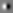
\includegraphics[width=0.2\columnwidth]{\figpath/Gx} &

\includegraphics[width=0.2\columnwidth]{\figpath/Gxx} &
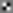
\includegraphics[width=0.2\columnwidth]{\figpath/Gxy} &

\includegraphics[width=0.2\columnwidth]{\figpath/Gxx-Gyy} \\
(a) & (b) & (c) & (d) \\
\noalign{\smallskip}
%
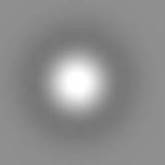
\includegraphics[width=0.2\columnwidth]{\figpath/mono_b} &
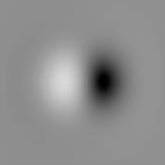
\includegraphics[width=0.2\columnwidth]{\figpath/mono_hx} &
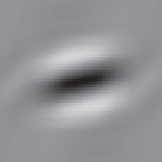
\includegraphics[width=0.2\columnwidth]{\figpath/dt_cwt_r4} &
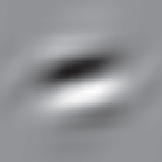
\includegraphics[width=0.2\columnwidth]{\figpath/dt_cwt_c4} \\
(e) & (f) & (g) & (h) \\
\noalign{\smallskip}
\end{tabular}
%
\caption{(a)~First derivatives $\Gx = \Gy^T$; (b-d)~Second derivatives, $\Gxx = \Gyy^T$, $\Gxy$; and $\Gxx-\Gyy$; (e,f)~Monogenic signal filters $B$ and $h_x = h_y^T$; (g,h)~Real and complex responses of the \dtcwt~ $15^\circ$ subband.}
\label{f:filters}
\end{figure}


\subsection{Incorporating Local Phase}
\label{s:phase_filters}
Although filters based on second derivatives can give accurate output when positioned at the centre of a line feature, accuracy away from the centre of the line cannot be assured, and indeed the orientation will be ill-defined when centred on an asymmetric feature (such as an edge), as with first derivatives at line centres. Intuitively, we can see that an approach using both odd and even filters -- or more formally, accommodating variation in \emph{phase} of the filter -- would be preferable.

\comment{This is where using both sine and cosine parts of the Gabor filters is useful. We can largely ignore this, however, on grounds that Gabor filters are very expensive to compute.}

\comment{If we need the space, I'd consider reducing this to a paragraph that states that the monogenic signal suffers the same problems as first derivatives, despite its use of phase.}
The monogenic signal~\cite{Felsberg_Sommer_TSP01} does this using three filters: one even band-pass filter $B$, and an odd quadrature pair of filters $h_x(x,y) = x/f(x,y)$ and $h_y(x,y) = y/f(x,y)$ where $f(x,y) = 2\pi(x^2 + y^2)^{\frac{3}{2}}$ (\fref{f:filters}e-f). These filters are combined to compute local amplitude~($A$), phase~($\psi$) and orientation~($\theta$) at each location in the image:

\begin{align}
A       &= \sqrt{{I_B}^2 + {I_{hx}}^2 + {I_{hy}}^2} \label{e:ma} \\
\psi	  &= \tan^{-1}\left[ \frac{I_B}{\sqrt{{I_{hx}}^2 + {I_{hy}}^2}} \right] \label{e:mp} \\
\theta  &= \tan^{-1}\left[ \frac{I_{hy}}{I_{hx}} \right] \label{e:mt}
\end{align}

\noindent where $I_{hi} = h_i \ast I_B$ in a slight abuse of our earlier notation.
\comment{define Ib, Ihx and Ihy}

In this context, the local amplitude provides a magnitude of response consistent for all structures and orientations. Meanwhile the local phase provides a measure of symmetry (in a profile of the structure perpendicular to its orientation), varying from $-\pi/2$ for a negative line (i.e. a dark line on a light background), $0$ for an edge and $\pi/2$ for a positive line.

However, in \eref{e:mt}, we again see a flaw in estimating orientation at the centre of a line. Because the even filter $B$ is isotropic, the only directional information we obtain is from the odd filters $h_x$ and $h_y$, thus as with Gaussian first derivatives the orientation at the centre of a line is ill-defined. In section~\ref{s:expts_retinography}, we show the debilitating effect this has on performance in real images.

Consequently, we would prefer a scheme in which odd and even filters are applied directionally. Historically, Gabor filters (combining both sine and cosine functions with a Gaussian kernel) have been a popular choice~\cite{Daugman_TASSP88}. However, these are neither steerable nor separable and therefore the cost of computing multiple oriented filters across several scales and storing the resulting coefficients is impractical for datasets of large images.

\comment{We leave Gabor filters, not only because they are computationally intensive but also because of the extra free parameter (angular resolution) that will affect the accuracy of the estimated orientation}

Instead, we propose using the Dual-Tree Complex Wavelet Transform (\dtcwt~\cite{Kingsbury_PTRSLA99}). The \dtcwt~has advantages over similar methods in that it combines the computational efficiency of decimation (\ie~multiresolution filtering is achieved by successively down-sampling the image by factors rather than by increasing filter size) whilst using separable filters and still producing approximately shift-invariant coefficients. Though further details on the construction of the \dtcwt~are beyond the scope of this paper, for our purposes it suffices to know that, at each scale, the transform generates a complex response at each of six angles (approximately $\pm15^\circ$, $\pm45^\circ$ and $\pm75^\circ$), where the real and imaginary parts are the responses to a pair of filters with phase $90^\circ$ apart (\fref{f:filters}g-h). The resulting decomposition has redundancy of just 4:1 and thus it is practical to store the decomposition of even large images such as mammograms. The decimated coefficients can then be interpolated at any spatial location (e.g. at points on the original pixel grid).

However, decimation introduces further complications because the filters will not necessarily be computed centrally over structures of interest. As such, the phase of \dtcwt~coefficients in the support of a structure encode both the symmetry of the structure and a spatial offset. By computing phase differences both spatially and across scale, it is possible to recover local phase that is globally consistent for structure symmetry (and analogous to the phase returned from the monogenic signal) and analytically compute local orientation (\cite{Anderson_ICP05,Anderson_ILP05}).

Alternatively, the coefficients may be passed directly into a suitably trained regressor to estimate orientation~\cite{Berks_etal_IPMI11} and this is the approach we explore further in this work. To achieve $180^\circ$ rotational symmetry, we replace any coefficient with negative imaginary part with its complex conjugate (equivalent to taking the absolute value of the local phase) and adjust the six sub-bands such that the phase at the centre of the impulse response of each wavelet is zero~\cite{Kingsbury_ECSP06,Berks_etal_IPMI11}.

\comment{When dealing with a complex response, $c$, we separate its magnitude, $|c|$, from its phase, $\angle c$. Since orientation is only defined up to a rotation of $180^\circ$, however, a point with phase $\phi$ displaced by $d$ from the centre of a line is indistinguishable from a point with phase $-\phi$ displaced by $-d$ from the same line when looking in the opposite direction; we therefore take the absolute value of phase, $|\angle c|$, at each pixel.}


\subsection{Multiscale Filtering}
Since curvilinear structure appears at a number of scales in the image (\eg~from fine spicules to thick ducts in mammograms), it necessary to filter the image at several scales to capture all structure~\cite{Lindeberg_IJCV98b}. For the first and second derivative methods this is achieved  by varying the width of the Gaussian kernels applied to the full-size image, whilst for the Monogenic signal suitable choices of the isotropic bandpass filter $B$ must be chosen. In contrast, multiresolution filtering is implicit in the decimated decomposition of the \dtcwt.

Having obtained responses at a number of scales, we must decide how to interpret them to produce a single estimation of orientation. One option is to discard all scales but that with the strongest overall response~\cite{Karssemeijer_teBrake_TMI96} and use the responses from the discrete orientations at the selected scale to determine orientation analytically. In this work, however, we investigate the alternative approach whereby we use the responses at all scales as input to a regressor that predicts the orientation directly. \comment{This general purpose approach has the added advantage that it can be applied for filter banks where an analytic solution is not obvious (such as the \dtcwt).}


\section{Estimating Orientation via Learning}
\label{s:learning}
If we have examples of labelled image data for which we wish to estimate orientation, a sensible approach is to compute filter responses (\ie~that form a feature vector) at sampled points in these images and train a regressor to predict the corresponding orientation. We can then apply the trained regressor to a previously unseen image in order to estimate orientation in new cases. Not only is this approach beneficial where an analytic solution is not obvious (as in the \dtcwt) but it also provides a simple method for pooling responses over scales and in a local neighbourhood, and accounts for factors such as the expected distribution of line widths in a typical image and non-Gaussian noise in medical imaging applications.

For the three regressors we use, the targets that we predict are a unit vector in the complex plane where the angle has been doubled (\ie~$t_k = \cos 2\theta_k + i\sin 2\theta_k$) to avoid ambiguity over direction~\cite{Mardia_Jupp_00}. Except where stated otherwise, we define the feature vector at a pixel as the responses to all filters pooled over the surrounding $3{\times}3$ pixel region.


\subsection{Linear Regression}
\label{s:learning_linear}
As a simple baseline, we use a linear regressor such that the predicted output is a weighed sum of the filter responses. Because the outputs are complex the regression coefficients are complex also, though this problem is equivalent to regressing over $\cos 2\theta$ and $\sin 2\theta$ independently.

\comment{We may want to reintroduce a note here that there are two solutions to the orientation, and that this cannot be estimated from a linear regression alone (at least for the double angle representations)}

%Under ideal conditions, applying this method to the real filters (\eg~first and second derivatives) should produce regression coefficients identical to those computed analytically.\comment{Not sure if that is entirely relevant}

%Since the linear regressor minimizes the mean squared error (in $\cos 2\theta$ and $\sin 2\theta$), the uncertainty in the prediction can be represented as an axis aligned Gaussian distribution in the complex plane. If the errors are equally distributed for both $\cos 2\theta$ and $\sin 2\theta$ -- and our experience suggests that they are typically close -- then the angular error (\ie~the angle subtended by isocontours of the Gaussian) is constant for an input of given magnitude; uncertainty is proportionally lower for inputs with larger magnitude, and vice versa. Since phase is limited to the range $[-\pi,\pi)$, however, the magnitude of the feature vector is strongly correlated with the magnitude (rather than phase) of the response to the \dtcwt. As a result, image features with high contrast that respond strongly to the \dtcwt~have lower relative uncertainty (an intuitive result).\comment{This could be considered as 'discussion' and may not be relevant right here}


%\subsection{Logistic Regression}
%\label{s:learning_logistic}
%Since we are predicting sin2T and cos2T, it makes sense to apply some limits to the values these can take. One possibility is to us logistic regression (usually used for classification) which can model a linear region for appropriately scaled targets or a sigmoidal output if necessary. We scale sin and cos to the range [0,1] to learn the regressor and apply the reverse transform on the predictions. This does not restrict outputs to be on (or within) the unit circle but within the unit square.
%
%This is slower to train since it requires iteratively reweighted least squares to minimize the objective function though adds little to testing times.
%Uncertainty will be tricky here


\subsection{Boosted Regression}
\label{s:learning_boosted}
Though straightforward, linear regression breaks down if the relationship between inputs and outputs is in fact nonlinear. Furthermore, the output of a linear regressor is unbounded even though in reality $-1 \leq \sin\theta,\cos\theta \leq 1$. We therefore investigate additive (or \emph{boosted}) regression models that can not only limit output but also capture any nonlinearities in the relationship between feature vector and orientation.

In this work we use an additive model composed of $N=100$ piecewise constant functions. To train the model, we start with a zero residual and iterate the following steps $N$ times: fit a weak predictor to each dimension of the training data in turn; select the dimension and corresponding predictor that minimize the residual error; add a fraction (we use $0.05$) of the prediction to the estimated outputs -- a process known as \emph{shrinkage}~\cite{Friedman_AoS01}; and recompute the residual error. This boosting process is thought to be more insensitive to overtraining than most Machine Learning methods.


\subsection{Random Forest Regression}
\label{s:learning_forest}
Random forests have been shown to be capable of learning complex nonlinear relationships over large numbers of variables (with absolute scales that are incommensurate) at a reasonable computational cost~\cite{Breiman_ML01}. Furthermore, they require little or no tuning and are often resistant to overtraining, making them ideally suited to our regression task. In this setting, a forest consists of $N=200$ binary regression trees each of which is built from a bootstrap sample of the training data. At each tree node, an optimal split is determined from only a random subset of the possible feature dimensions (rather than assessing all feature dimensions as in a standard tree algorithm).

We must be cautious, however, when using trees to predict orientation where vectors close to each other in the complex plane (\eg~$-1+\epsilon i$ and $-1-\epsilon i$) may be confused as being far apart based on their angle alone. Moreover, splitting dimensions and thresholds are usually chosen based on the variance of the sample either side of the threshold under the assumption of a input Euclidean space.
\comment{One reviewer complained about this previous sentence}%
As this assumption does not apply to orientation vectors, we instead use the angular dispersion~\cite{Mardia_Jupp_00}: for a sample of $N$ orientations $\{\theta_k\}$, represented in angle-doubled vector form as $t_k = \cos 2\theta_k + i\sin 2\theta_k$, the angular dispersion, $D$, of the sample can be defined as the magnitude of the mean vector over the sample \ie~$D = |(\sum{t_k})/N|$.
%
%\begin{equation}
%D = |\frac{\sum{t_k}}{N}|
%\label{e:2d}
%\end{equation}
%
By definition, $D$ reaches its maximum of 1 when all $t_k$ are equal, and its minimum of 0 when orientations are distributed uniformly about the circle or when the sample consists of pairs exactly $180^\circ$ apart. The aim of each regression tree is thus to find parts of the input feature space that are associated with pure samples of orientation. As such we implement our splitting criteria so that the sum of the angular dispersions of the two samples produced by the split is maximised.

We have found, however, that rather than constructing trees until completely pure leaves are found (\ie~nodes with $D$ arbitrarily close to 1), it is both computationally more efficient and more robust to stop when some minimum leaf size is reached (typically 0.05\% of the total input samples). We then store the mean sample vector of orientations at each leaf, in effect encoding a summary description of the sample of orientations at that point in the feature space (\ie~a mean orientation and an angular dispersion). The magnitude of these vectors can be viewed as the confidence in a leaf's ability to predict orientation.

When we apply the regression forest to predict orientations, we take the mean of the prediction vectors from the individual trees. Thus trees which described the input feature poorly (and so return a leaf orientation vector with small magnitude) contribute little to the overall orientation prediction, relative to trees that were able to match the input feature to a pure sample of orientations. Implementing forests in this way produces orientation predictions that are both more accurate and more robust (\ie~resistant to overtraining) than those from unpruned trees with uniform weighting of leaf orientations.

The magnitude of the final prediction can be viewed as measure of forest's confidence in the estimated orientation. This can be used in further processing and is also useful for weighting predictions in visualization (see \fref{f:real_mammography}).
%Previous work has looked at detecting structure by applying random forest classifiers to \dtcwt based feature vectors and we are currently exploring the link between two. \comment{ possibly cite our earlier work or reyhaneh's stuff - I promise I'm not doing this just self cite, it seems genuinely relevant!}


\comment{
\item When estimating orientation with a tree (or forest of trees), there is a particular problem when the output is limited to a specific range e.g. (0,2pi]. At the two extremes of the range, samples in the bins near the end are biased toward the centre of the range such that, in our case, it is very unlikely that a 0 or 2pi will be output by the forest.
Random Forests (or trees for that matter) have the option of giving us a multimodal distribution over orientation which will be useful at points where lines cross.
One advantage of the (pruned) tree approach is that each bin contains a number of training samples such that we can estimate a mean value and an uncertainty (variance) for every leaf. In other words, the variance is very much data dependent.
This then propagates in the case of a Random Forest since the individual tree outputs can be combined with their respective variance accounted for correctly.
The output from the Random Forest is always between 0 and 1 in magnitude. Question: should we be taking the square root of the complex vector to halve the angle (and therefore sqrt the magnitude also)? At the moment, vectors are weighed by their unsquared magnitude.
}


\section{Experiments}
\label{s:expts}
In our first set of experiments, we present a quantitative evaluation of the three regressors on real retinography images and mammogram-like data for which we have ground truth. We also present qualitative results on real mammography images for which ground truth was not available.
\comment{Are differences statistically significant?}


\subsection{Real Retinographic Images}
\label{s:expts_retinography}
The publicly available DRIVE dataset~\cite{Staal_etal_TMI04} contains 40 full colour retinogram images (\fref{f:retinography}a) of $565{\times}584$ pixels, split into 20 training and 20 test images. A hand-labelled mask that indicates vessel pixels (\fref{f:retinography}b) is also available for every image, enabling us to skeletonize the mask and approximate ground truth, $t_{gt} = \cos 2\theta_{gt} + i\sin 2\theta_{gt}$, from the skeleton for every labelled pixel.\comment{It is questionable how well this constitutes ground truth}

For training, we first transformed all images to monochrome via a weighted sum of the three RGB channels (though using only the green channel is also popular). We then selected 200\,000 vessel pixels randomly over the training set and computed filter responses to the first and second derivatives of a Gaussian (\fref{f:filters}e-f), the Monogenic signal filters (\fref{f:filters}g-h) and the \dtcwt~for every selected pixel. We used the resulting 200\,000 feature vectors and their corresponding target orientations to train each of the three regressors.
\comment{Why 200k points? Was this limit dictated by system requirements?}

During testing, we applied each regressor in turn to estimate the complex orientation, $t_{est} = \cos 2\theta_{est} + i\sin 2\theta_{est}$, at every pixel for every test image (\fref{f:retinography}c) and computed the orientation error with respect to ground truth,
%
\begin{equation}
	\theta_{err} = \frac{|\angle(t_{gt} \cdot t_{est}^*)|}{2}
\end{equation}

\noindent at labelled vessel pixels in the test image mask, where $t_{est}^*$ is the complex conjugate of $t_{est}$.

\begin{table}[tb]
\centering
\input{retinogram_table.txt}
%
\caption{Median absolute error in degrees for images 01-20 of the DRIVE database of retinal images. Results are shown both for the whole vessel and (in brackets) along the centre of the vessel only. These are given over different window sizes ($1{\times}1$ and $3{\times}3$) for first ($G'$) and second ($G''$) derivatives of gaussians, the monogenic signal, and the dual tree complex wavelet transform. Each feature type is used to predict orientation using the analytic solution (except for the \dtcwt), linear regression, Boosted regression and Random Forest regression.}
\label{t:retinopathy}
\end{table}

\begin{figure*}
\centering
\begin{tabular}{@{}c c c@{}}
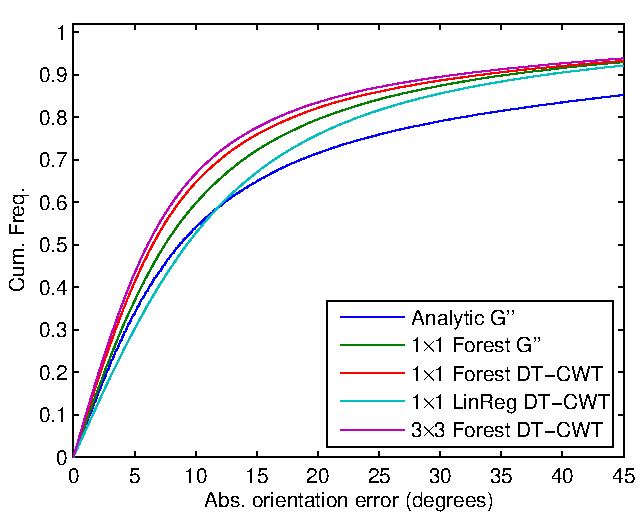
\includegraphics[width=.3\textwidth]{\figpath/retina/cumfreq} &
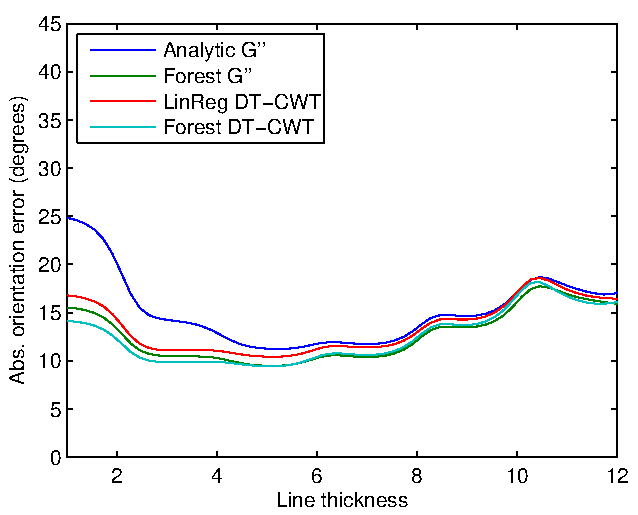
\includegraphics[width=.3\textwidth]{\figpath/retina/thickness_vs_error-summ} &
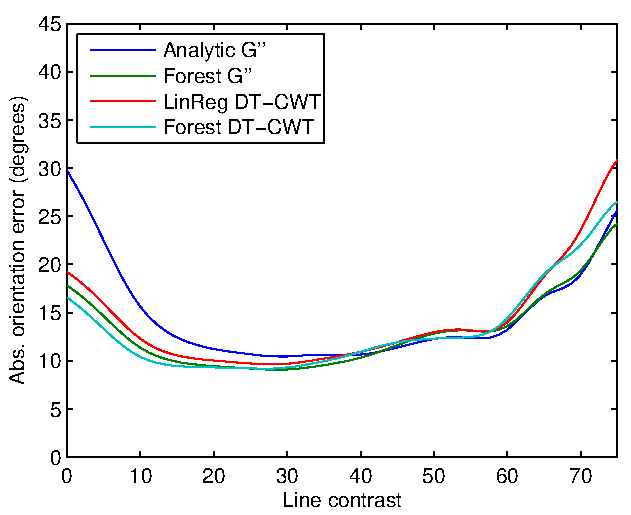
\includegraphics[width=.3\textwidth]{\figpath/retina/contrast_vs_error-summ} \\
(a) & (b) & (c) \\
\noalign{\smallskip}
\end{tabular}
%
\caption{Retinogram results for five selected methods over pixels along the centre of the vessel: (a) Cumulative frequency of angular error; (b) Kernel estimate of mean error with respect to line thickness; (c) Kernel estimate of mean error with respect to line contrast.}
\label{f:retina_graphs}
\end{figure*}

\comment{Some measure of spread for these figures, or a box plot to show significance.}

To compare the performance of different features and regressors, we computed median errors over both the whole vessel, and over the centre line only (\tref{t:retinopathy}).\footnote{The median is more robust than the mean to outliers in the error distribution.} Because faint, narrow vessels are the most challenging (and interesting), we also compare estimated errors for five selected methods over a range of line widths and contrasts (\fref{f:retina_graphs}). Line width was estimated from the distance transform of the vessel mask, whereas line contrast was measured as the absolute difference between the vessel intensity and the mean intensity of background pixels in a $15{\times}15$ neighbourhood.

\paragraph{Choice of feature}
Features based on odd filters (\ie~first derivatives of the Gaussian and the monogenic signal) were consistently outperformed by those that included even filters. This can be attributed to the high errors that occur when using only odd filters at the centre of a vessel where there is little or no image gradient; this failure is particularly acute for the most narrow vessels, consisting of a single pixel, where the whole vessel is a centre-line by definition. Of the two features that use even filtering -- the second Gaussian derivatives and the \dtcwt~-- the \dtcwt~provided better estimates under most conditions. This suggests that using both odd and even filters (such that phase information becomes available) does indeed improve performance, though at a cost in computational demand.

\paragraph{Choice of regressor}
Our use of learnt regressors was motivated by their ability to pool over scales and local neighbourhoods, to combine filter responses where an analytic solution was not obvious (\eg~when using the \dtcwt), and to model data-dependent properties such as image noise and the observed distribution of line widths and contrasts. In almost all cases (excepting some linear regression conditions) this was confirmed by the results: errors produced by the learnt regressors were lower than those achieved using an analytic solution, often in proportion to the complexity of the classifier. In particular, Random Forests achieved consistently lower error rates than the other classifiers.

As noted earlier, when using second derivative responses it is necessary to compute the responses at the two possible solutions to determine which is the correct one. Since the linear regressor minimizes the average error, however, it contains no mechanism for selecting the correct orientation and this is likely to be one reason for its poor performance relative to more sophisticated regressors such as the Random Forest.

\paragraph{Choice of window size}
Pooling results over a local neighbourhood by stacking filter responses into a single vector also had a significant effect on error rates. This was particularly the case for features based on odd filter responses, since it reduces the effect of small gradients at the centre-line by pooling estimates from nearby pixels with stronger gradients and therefore better estimates.

As an aside, we also note that second Gaussian derivatives can be closely approximated using finite differencing of a first Gaussian derivative. Therefore, a linear regression over first derivative responses at neighbouring pixels is able to replicate the errors of the method based on second derivatives.

\paragraph{Effects of line thickness}
Though it is clear that a learnt regressor produces lower errors than a prescribed analytic solution when averaged over all vessel points, it is also helpful to look at how errors are distributed with respect to line parameters such as vessel thickness. We visualize this relationship using a one dimensional kernel smoother (\fref{f:retina_graphs}b), and see that errors are similar for the thicker vessels (where there is more image information with which to estimate orientation and thus we expect all methods to perform well) but that the regression reduces error considerably for the narrower vessels. Interpreting results for vessels with a width of more than approximately 12 pixels is difficult because they are rare, which leads to high variability in the kernel estimate of error, and because the vessel width exceeds the central region of our largest filter. These vessels, however, are typically of less interest to the retinopathy community.

\paragraph{Effects of line contrast}
We see a similar effect when considering the distribution of error with respect to line contrast (\fref{f:retina_graphs}c): the learnt regressors outperform analytic methods especially on lines with low contrast though there is little significant difference between the methods for vessels of greater contrast. We also see errors begin to increase beyond a certain contrast, though this is most likely due again to the rarity of high contrast vessels and the correlation of high contrast with large width.

\subsection{Mammogram-like Images}
\label{s:expts_synth_mammography}
As vessels are often clearly visible in retinograms, we repeated this experiment on a more challenging dataset of synthetic images that realistically approximate the structure of mammographic images. More specifically, we sampled a background by cropping a $512{\times}512$ image region from a real mammogram upon which we superimposed one or more lines of varying orientation, contrast, width and profile. As the lines were synthetic, we had access to ground truth orientation for the superimposed structure. Unlike other similar studies~\cite{Berks_etal_IPMI11}, we do not require a negative classification of background pixels and therefore do not need to remove existing real structures from the images. As a result, the synthetic lines will be disrupted by any existing image structure and thus the dataset presents a much tougher and more realistic test of orientation estimation than shown in, for example,~\cite{Berks_etal_IPMI11}.

\begin{table}[t]
\centering
\begin{tabular}{l c c c c}
\toprule
							& \multicolumn{4}{c}{Feature Type} \\
							& $G'$		& $G''$	& Mono.				& \dtcwt \\
\cmidrule{2-5}
\input{mammography_table.txt}
\bottomrule
\noalign{\smallskip}
\end{tabular}
%
\caption{Median absolute error (degrees) for combinations of input feature and {3{$\times$}3} regressor on 100 synthetic mammogram images.}
\label{t:synth_mammography}
\end{table}

\begin{figure}[t]
\centering
\begin{tabular}{c c}
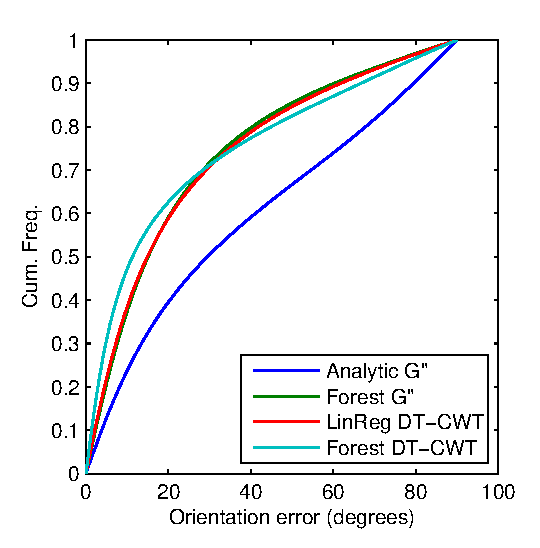
\includegraphics[width=0.47\columnwidth]{\figpath/mammo/cdf_error_mammo} &
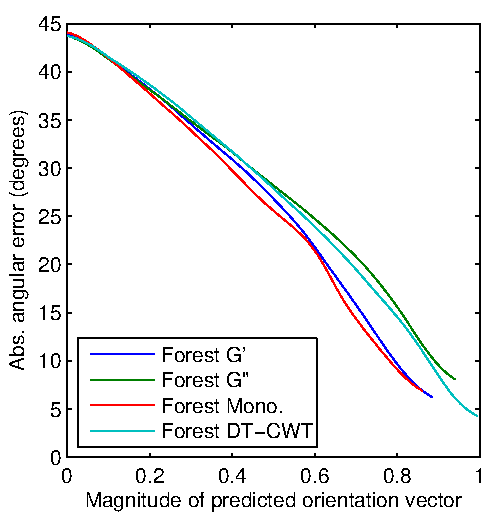
\includegraphics[width=0.46\columnwidth]{\figpath/mammo/response_vs_error_mammo} \\
(a) & (b) \\
\noalign{\smallskip}
\end{tabular}
%
\caption{Mammogram results for four selected methods: (a) Cumulative frequency of angular error; (b) Kernel estimate of mean error with respect to the magnitude of the orientation vector predicted by the forest.}
\label{f:mammo_graphs}
\end{figure}

As in the retinogram experiment, we sampled 200\,000 pixels from such images and computed a feature vector for each with which we trained a regressor. We then applied every trained regressor for every feature type to a fixed set of 100 synthesized images (generated from mammographic backgrounds not used in training)  and computed the error at the known line pixel positions. As before, Random Forests and the \dtcwt~outperform other methods, though errors were generally higher on account of the more challenging data (\fref{f:mammo_graphs}a and \tref{t:synth_mammography}). We also note that although the median error for the Random Forest was lower for the \dtcwt~than the second derivatives, the situation was reversed for higher percentiles (\ie~the graphs cross). We care less, however, about differences between errors above a certain threshold (it matters little whether the estimate is out by $60^\circ$ or $70^\circ$ -- they are both terrible estimates) so it may be argued that the Random Forest performs better over the region in which we are interested.

In \fref{f:mammo_graphs}b we show the kernel estimate of mean angular error with respect to the magnitude of the orientation vector predicted by the forest trained on each feature type. Recall that this magnitude encodes the mean angular dispersion of the training data arriving the leaf nodes used in making each orientation prediction. That this magnitude acts as a measure of confidence in its prediction is evidenced by consistent reduction in angular error with increasing magnitude for all feature types. The magnitudes can be used to weight each orientation prediction in further processing and may be preferable to a similar feature such as the absolute response returned from the analytic combination of the Gaussian derivatives. This is because the latter is essentially a measure of image contrast at a structure of interest. So for example, if there are two lines, one of which has double the contrast of the other, the magnitude of the filter response will also double, even if the orientation may measured equally accurately in both lines. Similarly, a very bright or very dark spot in the image will also produce a strong filter response where in fact orientation can't be reliably estimated.

Having trained regressors on synthetic mammogram-like images, we can also apply them to real mammograms. Qualitative analysis of the results predictions verifies that the training data acts as a suitable surrogate for real data (although we would expect better predictions if ground truth labelled real data were available). For example, in a region of interest surrounding a spiculated lesion (\fref{f:real_mammography}a), the linear structures radiating from the central mass are clearly visible in the resulting orientation predictions weighted by the prediction confidence (\fref{f:real_mammography}b).

\begin{figure}[t]
\centering
\begin{tabular}{@{}c c@{}}
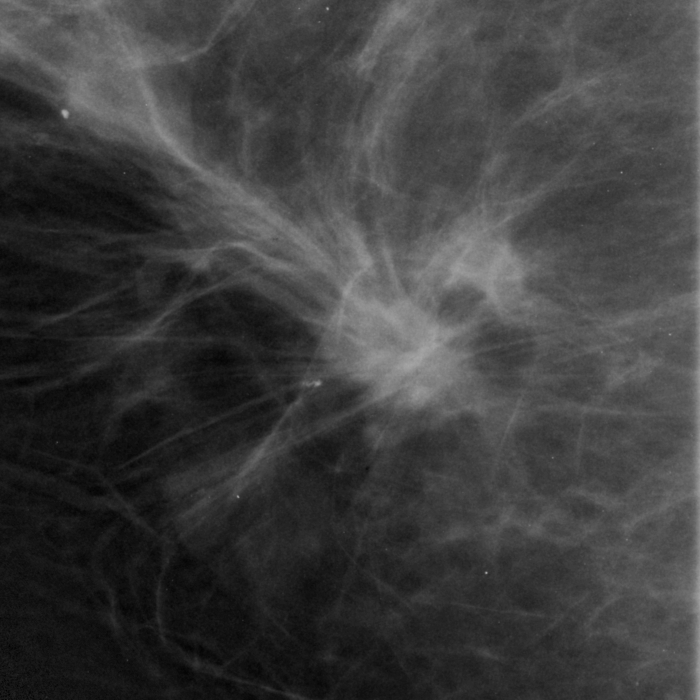
\includegraphics[width=0.47\columnwidth]{\figpath/mammo/024RCC_roi_crop} &
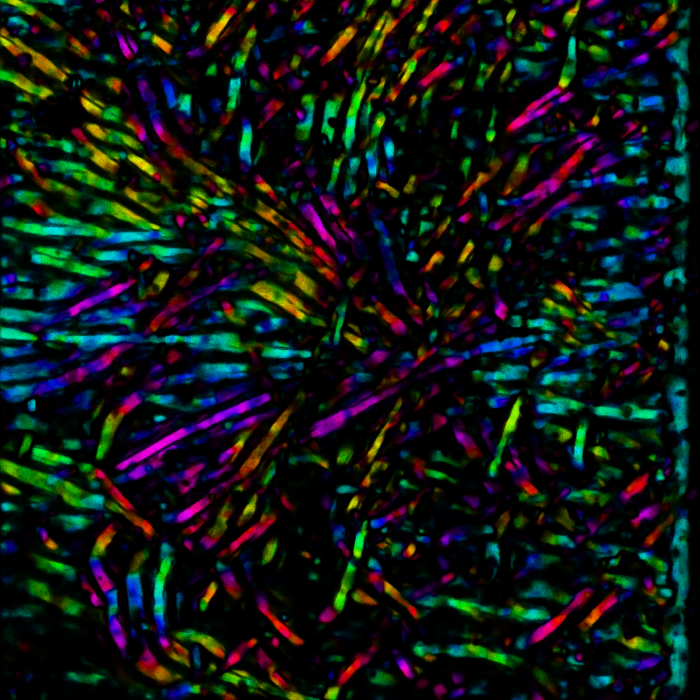
\includegraphics[width=0.47\columnwidth]{\figpath/mammo/024RCC_roi_class_ori_crop} \\
(a) & (b) \\
\noalign{\smallskip}
\end{tabular}
%
\caption{Real mammographic images: %
(a) input image; %
(b) estimated orientation from a Random Forest using \dtcwt~features. Hue indicates the estimated orientation and brightness is determined by the confidence in the estimate (as quantified by the magnitude of the predicted orientation vector).}
\label{f:real_mammography}
\end{figure}

% CLAIM: that the separable filters are faster than nonseparable ones (but by how much?)
% CLAIM: that the Haar-like features are faster than separable filtering
In terms of efficiency, we recorded the mean time (using Matlab on a 2.66Ghz, quad-core desktop PC with 3.25Gb RAM) over 20 images for three feature representations: the monogenic signal (2.96s); second derivatives (2.04s); and the \dtcwt (19.96s). Unsurprisingly, under test conditions the \dtcwt~was an order of magnitude slower than the separable filters. %*The Haar-like approximations were comparable to but slower than the separable filters, though the separable filters did exploit the built-in (\ie~compiled) convolution functions in Matlab; we expect that an optimized implementation of the Haar-like features would offer similar performance gains as observed in face detection applications~\cite{Viola_Jones_IJCV04}.*/
%%% This is a pretty weak conclusion to the experiment but the best we can expect at this point. Also, if you need to use a regressor as slow as the RF to get accuracy that is comparable to the analytic second derivatives then the small difference in filtering time becomes irrelevant}


%\subsection{Fingerprint Analysis}
%\label{s:expts_fingerprints}
%Noting that estimating orientation is of interest to the fingerprint analysis community, we briefly present some results that highlight the difference in performance between using filters based on first and second derivatives, respectively. As discussed earlier, the estimated orientation using gradient based filters~\cite{Bazen_Gerez_TPAMI02,Mei_etal_IVC09} -- the mainstay of fingerprint orientation analysis -- becomes unstable near the centre of a symmetric bar feature (\fref{f:fingerprints}b), whereas a filter based on second derivatives remains stable (\fref{f:fingerprints}c). There are, however, artefacts around the edges of the ridge features for the second derivative that may suggest a solution based on both types.

%\begin{figure}[t]
%\centering
%\begin{tabular}{c c c}
%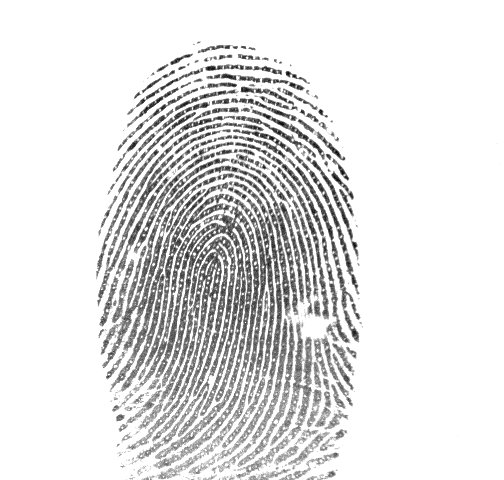
\includegraphics[width=0.3\columnwidth]{\figpath/fingerprint/input} &
%%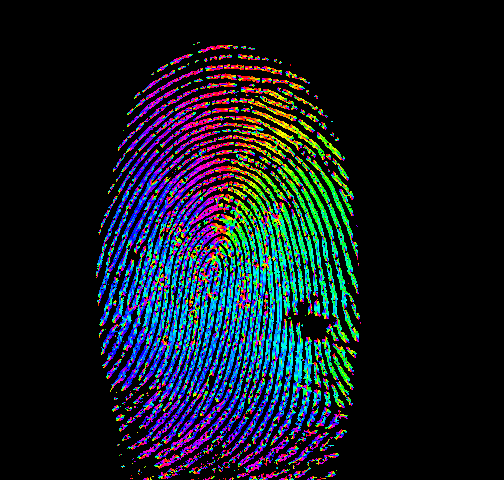
\includegraphics[height=0.15\textheight]{\figpath/fingerprint/ori_1st} &
%%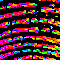
\includegraphics[height=0.15\textheight]{\figpath/fingerprint/ori_1st_zoom} \\
%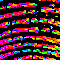
\includegraphics[width=0.3\columnwidth]{\figpath/fingerprint/ori_1st_zoom} &
%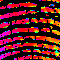
\includegraphics[width=0.3\columnwidth]{\figpath/fingerprint/ori_clover_zoom} \\
%(a) & (b) & (c) \\
%%&
%%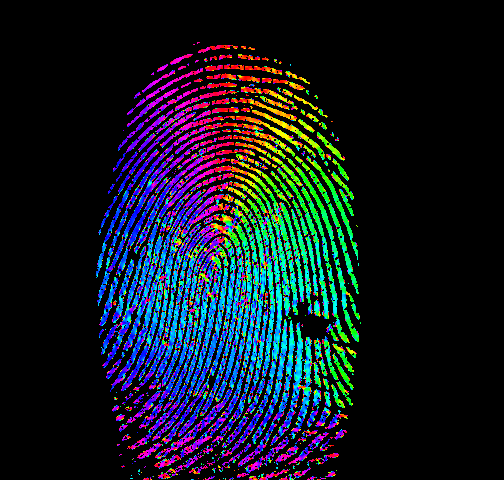
\includegraphics[height=0.15\textheight]{\figpath/fingerprint/ori_clover} &
%%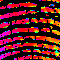
\includegraphics[height=0.15\textheight]{\figpath/fingerprint/ori_clover_zoom} \\
%%		& (d) & (e)
%\end{tabular}
%%
%\caption{Fingerprint images: %
%(a) input image; %
%(b,c) first derivative estimate of orientation with close-up; %
%(d-e) second derivative estimate with close-up. Note the high errors at the centre of the ridge for first derivatives and at the edges of the ridge for second derivatives.}
%\label{f:fingerprints}
%\end{figure}


%\section{Discussion}
%\label{s:discussion}
%
%\begin{figure}[t]
%	\centering
%		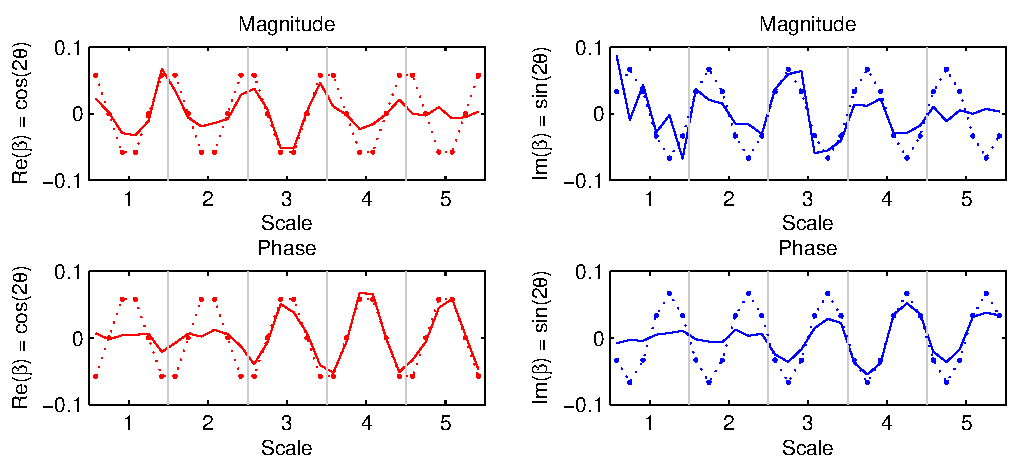
\includegraphics[width=0.9\columnwidth]{\figpath/linreg_coeffs}
%	\caption{Linear regression coefficients for (left) $\cos 2\theta$ and (right) $\sin 2\theta$, using (top) response magnitude and (bottom) response phase.}
%	\label{f:linreg_coeffs}
%\end{figure}



\section{Conclusions}
\label{s:conclusions}
In conclusion, we see that filters based only on odd filters perform poorly near the centre of a curvilinear structures; even filters such as the second derivatives are much better, although a feature set comprising the responses to both odd and even filters offers further advantages. Of the filters we tested, we found that the \dtcwt~gave the best results regardless of the regressor used, though was significantly more computationally expensive. Of the regressors we tested, Random Forests performed best and we have provided some insight as to why alternatives (\eg~linear regression) perform less well. Most promisingly, we note the larger improvement in orientation estimation for particularly challenging structures such as thin, low-contrast vessels. Moreover, when using Random Forests we propose that both the predicted orientation \emph{and} its associated magnitude may be useful features in further processing. \comment{We must, however, take care when building regressors for orientation prediction in order to ensure that angles wrap around the circle correctly.}

%\end{document}

\bibliographystyle{splncs}
\bibliography{./bib/_aliases,./bib/mobio,./bib/mammography,./bib/ml,./bib/local}

\end{document}

\clearpage
\appendix
\section{Derivations}
Defining $\G_{(1)}(\theta)$ as the first derivative filter at angle $\theta$,
%
\begin{align}
\G_{(1)}(\theta)
	&= 	\frac{\partial G}{\partial r} \\
	&= 	\frac{\partial G}{\partial x}\frac{\partial x}{\partial r} +
			\frac{\partial G}{\partial y}\frac{\partial y}{\partial r} \\
	&= 	\Gx \cos(\theta) + \Gy \sin(\theta)
\label{e:dG}
\end{align}

\noindent where $\Gx = \G_{(1)}(0^\circ)$ and $\Gy = \G_{(1)}(90^\circ)$ (\fref{f:filters}). We can write the response to this filter as
%
\begin{align}
R_{(1)}(\theta)
	&= 	\G_{(1)}(\theta) \ast I \\
	&=	(\Gx \cos(\theta) + \Gy \sin(\theta)) \ast I \\
	&=	(\Gx \ast I) \cos(\theta) + (\Gy \ast I) \sin(\theta)) \\
	&=	\Ix \cos(\theta) + \Iy \sin(\theta)
\label{e:R1}
\end{align}

\noindent such that differentiating and equating to zero gives
%
\begin{align}
\frac{d}{d\theta}R_{(1)}
	&= -\Ix \sin(\theta) + \Iy \cos(\theta) = 0 \\
\Rightarrow \tan(\theta)
	&= \frac{\Iy}{\Ix}.
\label{e:t1}
\end{align}



\begin{align}
R_{(1)}^2(\theta)
	&=	(\Ix \cos(\theta) + \Iy \sin(\theta))^2 \\
	&= 	\Ix^2 \cos^2(\theta)+\Iy^2 \sin^2(\theta)+2\Ix\Iy\sin(\theta)\cos(\theta) \\
	&= 	\Ix^2 \cos^2(\theta)+\Iy^2 \sin^2(\theta)+\Ix\Iy\sin(2\theta)
\label{e:R1sqr}
\end{align}

\noindent such that differentiating and equating to zero gives
%
\begin{align}
\frac{d}{d\theta}R_{(1)}^2
	&= 	-2\Ix^2 \cos(\theta)\sin(\theta) + 2\Iy^2 \sin(\theta)\cos(\theta) + 2\Ix\Iy\cos(2\theta) \\
	&= 	(\Iy^2-\Ix^2) \sin(2\theta) + 2\Ix\Iy\cos(2\theta) = 0 \\
\Rightarrow \tan(2\theta)
	&= 	\frac{2\Ix\Iy}{\Ix^2-\Iy^2}.
\label{e:t1sqr}
\end{align}


Squared filters:

\begin{align}
\tan(2\theta)
	&= 	\frac{2(\Gx\Gy \ast I)}{(\Gx^2 \ast I)-(\Gy^2 \ast I)}.
\label{e:t1fsqr}
\end{align}

\noindent with `cloverleaf' type filters.

Second derivs:
%
\begin{align}
\G_{(2)}(\theta)
	&= 	\frac{\partial}{\partial x}(\Gx \cos(\theta) + \Gy \sin(\theta))\frac{\partial x}{\partial r} +
			\frac{\partial}{\partial y}(\Gx \cos(\theta) + \Gy \sin(\theta))\frac{\partial y}{\partial r} \\
	&= 	(\Gxx \cos(\theta) + \Gyx \sin(\theta))\cos(\theta) +
			(\Gxy \cos(\theta) + \Gyy \sin(\theta))\sin(\theta) \\
	&= 	\Gxx\cos^2(\theta) + \Gyy\sin^2(\theta) + 2\Gxy\sin(\theta)\cos(\theta) \\
	&=	\Gxx\cos^2(\theta) + \Gyy\sin^2(\theta) + \Gxy\sin(2\theta) \\
\label{e:ddG}
\end{align}

\noindent where the response to this filter is
%
\begin{align}
R_{(2)}(\theta)
	&= 	\G_{(2)}(\theta) \ast I \\
	&=	\Ixx\cos^2(\theta) + \Iyy\sin^2(\theta) + \Ixy\sin(2\theta)
\label{e:R2}
\end{align}

\noindent with a stationary point at

\begin{align}
\frac{d}{d\theta}R_{(2)}
	&= 	-2\Ixx\cos(\theta)\sin(\theta) + 2\Iyy\sin(\theta)\cos(\theta) + 2\Ixy\cos(2\theta) \\
	&= 	(\Iyy-\Ixx)\sin(2\theta) + 2\Ixy\cos(2\theta) = 0 \\
\Rightarrow \tan(2\theta)
	&= 	\frac{2\Ixy}{\Ixx-\Iyy}.
\label{e:t2}
\end{align}


\end{document}
